%%
%% This is file `sample-sigconf.tex',
%% generated with the docstrip utility.
%%
%% The original source files were:
%%
%% samples.dtx  (with options: `all,proceedings,bibtex,sigconf')
%% 
%% IMPORTANT NOTICE:
%% 
%% For the copyright see the source file.
%% 
%% Any modified versions of this file must be renamed
%% with new filenames distinct from sample-sigconf.tex.
%% 
%% For distribution of the original source see the terms
%% for copying and modification in the file samples.dtx.
%% 
%% This generated file may be distributed as long as the
%% original source files, as listed above, are part of the
%% same distribution. (The sources need not necessarily be
%% in the same archive or directory.)
%%
%%
%% Commands for TeXCount
%TC:macro \cite [option:text,text]
%TC:macro \citep [option:text,text]
%TC:macro \citet [option:text,text]
%TC:envir table 0 1
%TC:envir table* 0 1
%TC:envir tabular [ignore] word
%TC:envir displaymath 0 word
%TC:envir math 0 word
%TC:envir comment 0 0
%%
%%
%% The first command in your LaTeX source must be the \documentclass
%% command.
%%
%% For submission and review of your manuscript please change the
%% command to \documentclass[manuscript, screen, review]{acmart}.
%%
%% When submitting camera ready or to TAPS, please change the command
%% to \documentclass[sigconf]{acmart} or whichever template is required
%% for your publication.
%%
%%
\documentclass[sigconf]{acmart}

%%
%% \BibTeX command to typeset BibTeX logo in the docs
\AtBeginDocument{%
  \providecommand\BibTeX{{%
    Bib\TeX}}}

%% Rights management information.  This information is sent to you
%% when you complete the rights form.  These commands have SAMPLE
%% values in them; it is your responsibility as an author to replace
%% the commands and values with those provided to you when you
%% complete the rights form.
\setcopyright{acmlicensed}
\copyrightyear{2024}
\acmYear{2024}
\acmDOI{XXXXXXX.XXXXXXX}

%% These commands are for a PROCEEDINGS abstract or paper.
\acmConference[Conference acronym 'XX]{Make sure to enter the correct
  conference title from your rights confirmation emai}{June 03--05,
  2018}{Woodstock, NY}
%%
%%  Uncomment \acmBooktitle if the title of the proceedings is different
%%  from ``Proceedings of ...''!
%%
%%\acmBooktitle{Woodstock '18: ACM Symposium on Neural Gaze Detection,
%%  June 03--05, 2018, Woodstock, NY}
\acmISBN{978-1-4503-XXXX-X/18/06}


%%
%% Submission ID.
%% Use this when submitting an article to a sponsored event. You'll
%% receive a unique submission ID from the organizers
%% of the event, and this ID should be used as the parameter to this command.
%%\acmSubmissionID{123-A56-BU3}

%%
%% For managing citations, it is recommended to use bibliography
%% files in BibTeX format.
%%
%% You can then either use BibTeX with the ACM-Reference-Format style,
%% or BibLaTeX with the acmnumeric or acmauthoryear sytles, that include
%% support for advanced citation of software artefact from the
%% biblatex-software package, also separately available on CTAN.
%%
%% Look at the sample-*-biblatex.tex files for templates showcasing
%% the biblatex styles.
%%

%%
%% The majority of ACM publications use numbered citations and
%% references.  The command \citestyle{authoryear} switches to the
%% "author year" style.
%%
%% If you are preparing content for an event
%% sponsored by ACM SIGGRAPH, you must use the "author year" style of
%% citations and references.
%% Uncommenting
%% the next command will enable that style.
%%\citestyle{acmauthoryear}


%%
%% end of the preamble, start of the body of the document source.
\begin{document}

%%
%% The "title" command has an optional parameter,
%% allowing the author to define a "short title" to be used in page headers.
\title{Ontology Construction for Database Statistics in Preparation for Learning Integration}

%%
%% The "author" command and its associated commands are used to define
%% the authors and their affiliations.
%% Of note is the shared affiliation of the first two authors, and the
%% "authornote" and "authornotemark" commands
%% used to denote shared contribution to the research.
\author{Leo Scott Fitzsimmons}
\affiliation{%
  \institution{Charleston Southern University}
  \city{North Charleston}
  \state{SC}
  \country{USA}
}
\email{lsfitzsimmons@csustudent.net}

\author{Songhui Yue}
\affiliation{%
	\institution{Charleston Southern University}
	\city{North Charleston}
	\state{SC}
	\country{USA}
}
\email{syue@csuniv.edu}

\author{Sean Hayes}
\affiliation{%
	\institution{Charleston Southern University}
	\city{North Charleston}
	\state{SC}
	\country{USA}
}
\email{shayes@csuniv.edu}
	
\author{Valerie Session}
\affiliation{%
	\institution{Charleston Southern University}
	\city{North Charleston}
	\state{SC}
	\country{USA}
}
\email{vsessions@csuniv.edu}


%%
%% By default, the full list of authors will be used in the page
%% headers. Often, this list is too long, and will overlap
%% other information printed in the page headers. This command allows
%% the author to define a more concise list
%% of authors' names for this purpose.
\renewcommand{\shortauthors}{Trovato et al.}

%%
%% The abstract is a short summary of the work to be presented in the
%% article.
\begin{abstract}
Ideally, researchers in the database areas and database administrators should easily reference statistics and other relevant metadata about their databases. However, extracting and presenting this statistical information in an easily consumable format typically demands significant effort and specialized skills. This research introduces an automated methodology for constructing and visualizing an ontology enriched with relational Database Statistics (DBS). By integrating collected metadata and statistics into a visually accessible database ontology graph, this approach enhances the ontology with the ability to support learning integration tasks such as ontology simplification, decision-making for database design and optimization, and ingestion by other artificial intelligence (AI) processes. The outcomes of this research include a methodology for augmenting database ontology graphs with statistical details, a proposed model for a DBS ontology, and use cases demonstrating potential learning integrations.
\end{abstract}

%%
%% The code below is generated by the tool at http://dl.acm.org/ccs.cfm.
%% Please copy and paste the code instead of the example below.
%%
\begin{CCSXML}
	<ccs2012>
	<concept>
	<concept_id>10002951.10002952.10003219.10003215</concept_id>
	<concept_desc>Information systems~Extraction, transformation and loading</concept_desc>
	<concept_significance>500</concept_significance>
	</concept>
	<concept>
	<concept_id>10002951.10003317.10003318.10011147</concept_id>
	<concept_desc>Information systems~Ontologies</concept_desc>
	<concept_significance>500</concept_significance>
	</concept>
	<concept>
	<concept_id>10002951.10003317.10003347.10011712</concept_id>
	<concept_desc>Information systems~Business intelligence</concept_desc>
	<concept_significance>300</concept_significance>
	</concept>
	</ccs2012>
\end{CCSXML}

\ccsdesc[500]{Information systems~Extraction, transformation and loading}
\ccsdesc[500]{Information systems~Ontologies}
\ccsdesc[300]{Information systems~Business intelligence}

%%
%% Keywords. The author(s) should pick words that accurately describe
%% the work being presented. Separate the keywords with commas.
\keywords{Ontology, Database, Statistics, Interoperability, Visualization}
%% A "teaser" image appears between the author and affiliation
%% information and the body of the document, and typically spans the
%% page.

%%
%% This command processes the author and affiliation and title
%% information and builds the first part of the formatted document.
\maketitle

\section{Introduction}
An ontology is a set of concepts and categories within a subject area or domain that defines their properties and the relationships between them. It forms the scaffolding that establishes standard terms, labels, and relationships, creating a common language for both structured and unstructured data \cite{gruber1993ontology, chari2020explanation}. Ontology allows for the processing and understanding of data upon the defined, common categorization of data and relationships \cite{yue2024csm}. One of the major objectives of ontology is to make knowledge in a domain computationally useful \cite{tudorache2020ontology}. For heterogeneous systems, it provides a common language by which disparate systems can communicate \cite{fraga2020ontology, yue2024csm}. For AI systems, it gives context to data and enables AI to “decide” based on content and relationship. Ontology graphs are a way to visually represent an ontology and increase learning and understanding of a domain. They provide a visual representation of relationships between classes, attributes, and properties \cite{gutierrez2018knowledge, yue2021applying}.

A multitude of resources (vendor documentation, domain experts' articles, and posts \cite{RWesta, RWestb, RWestc}) address RDBMS statistics maintenance (in this research, specifically Microsoft SQL Server© --or the rest of the document, referred to as “SQL Server”) and how the query optimizer uses statistics and histograms. The vast majority of the writings are functional and pragmatic, addressing how to solve issues related to performance. Academic work related to DBS and histograms is sparse; the limited information is curious because there are intricacies and subtleties to statistics updates and histograms, which make the query optimizer choose questionable plans that lead to poor and often unpredictable performance. Most efforts to resolve these issues are labeled and resolved as “statistics maintenance” problems and do not go much further. Furthermore, histogram data, primarily used by the query optimizer, are available to the analyst and have the potential for analysis and mining, but querying and presenting these data can be somewhat cumbersome and have a less-than-desirable default format.

The scarcity of information/research regarding DBS—specifically index utilization, column statistics, and histograms—and lack of deep study/mining into the same motivates this research. This effort first produces a statistics ontology to establish a standard ontology for DBS based on the subject matter knowledge of the RDBMS. It is intended for the ontology to define a domain and assist in making the statistics data “computationally useful.” The ontology shows DBS as they exist at different levels, taking opportunities to aggregate characteristics or flag important aspects. Next, with the resultant ontology in mind, a semi-automated process has been created and executed. The process produces two ontology graphs: an ontology graph centered on column statistics and an ontology graph based on index utilization. This transformation effort also produces enriching data in a supporting Hypertext Markup Language (HTML) document. Figure \ref{overview} below summarizes the full objective. The resultant ontology helps promote learning and establish a framework from which data can potentially be formatted for use by machine learning/AI.

\begin{figure}[h]
	\centering
	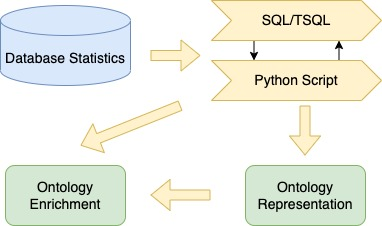
\includegraphics[width=0.8\linewidth]{db-statistics-ontology}
	\caption{An Overview of the Study.}
	\label{overview}
\end{figure}

This work contributes to DBS learning, reinforcing metadata concepts by visually organizing and representing statistics on appropriate object (table, index, column) levels. This work also contributes to statistics ontology (and, more specifically, database-related statistics) as it can be a starting point for future work regarding DBS modeling and mining opportunities using machine learning or other AI methods.

\section{Related Work}
There is a significant amount of research regarding ontology (in the scope of computer science) and the automatic/semiautomatic creation of ontology, especially as extracted from a relational database; the related works highlight many of these efforts, to include Protégé, RDB2OWL, and Mapping of Relational Schema \cite{christian2017mapping}. Deeper or specific understanding and learning are achieved by incorporating “enriching” data into the ontology, added in from an external source. Examples of automatic/semiautomatic ontology enrichment are the works by Booshehri and Luksch (using DBPedia as external source) \cite{booshehri2015ontology} and Rajput and Gurulingappa (using a unified medical language system) \cite{rajput2013semi}.

Creating an ontology can be very manually intensive and often requires domain expert involvement, so a great deal of research and effort has been given to automate the task of ontology creation. There are several research documents that summarize ontology approaches; for example, the approach in \cite{christian2017mapping} is very similar to this research, with at least the major difference of the RDBMS (Oracle) platform. The research conducted in the work of Loudi et al. \cite{louhdi2013hybrid} is also similar, using MySQL RDBMS. Būmans and Čerāns \cite{bumans2018rdb2owl} outline a process to map the database entities to Web Ontology Language (OWL) and includes a schema that may be used and/or improved. In these cases, the ontology was focused on a user schema/data, not statistics, and not toward a standardization or extraction of statistical metadata. 

\begin{comment}
	Issues common to building an ontology are the following:
	\begin{itemize}
		\item Domain experts needed for validation.
		\item Objects such as views may not translate into ontology, or important facts or relationships are sometimes missed.
		\item Ontology creation is dependent on the domain and the purpose of the ontology.
	\end{itemize}
\end{comment}

DBS, particularly in SQL Server, have been the subject of numerous white papers, conference sessions, blogs, and “best practices” lists. More specifically, the attention is more so on the maintenance of statistics due to their importance in accurately representing the actual data. Likewise, the primary purpose of the histogram is internal use; the query optimizer uses a column’s histogram to help estimate the number of rows a query will return. It is speculated that due to their functional nature and common perception of “internal use only” by the RDBMS, there is very little if any, academic-level research on column statistics and histograms. The work by Lee et al. \cite{lee2016operator} addressed the operation of SQL Server Live Query Statistics feature, but no other scholarly works have addressed or capitalized on the internal collections or analysis of statistics metadata.

\section{Motivation and Use Cases}
\begin{comment}
Efforts to generate ontologies from relational databases have successfully converted data definition language (DDL) output into OWL format. These ontologies serve as "knowledge scaffolding" that supports AI development by providing structured frameworks of concepts and relationships. Relational databases, due to their structured nature and comprehensive metadata, offer an effective platform for not only extracting data but also integrating business logic. 
\end{comment}
This research aims to achieve three primary objectives: producing a DBS ontology, generating statistics-centric ontology graphs enriched with data resources, and preparing the groundwork for data mining opportunities. Each of these motivations is elaborated upon below, with use cases embedded to demonstrate their practical relevance.

\subsection{Motivation 1: Produce a DBS Ontology}
Ontology, by definition, specifies a common vocabulary for a domain, facilitating information exchange between heterogeneous systems through semantic-level representation. This research aims to create a DBS ontology in XML format, visualized as an ontology graph via WebVOWL, as well as a regular diagram. The ontology will enhance understanding of DBS and their significance in evaluating database ontologies.

Use Case: An ontology defines a domain with common terms used by heterogeneous systems, and the creation of a DBS ontology aids in understanding what statistical information is available at different levels. For instance, a junior database administrator (DBA) tasked with comparing schemas from different databases may lack familiarity with DBS. Without the appropriate knowledge, they might resort to inefficient methods such as manually selecting counts from tables or researching distinct column values. By referencing the DBS ontology, the DBA can quickly comprehend what statistical data is available and at what object level, streamlining their tasks and enhancing their understanding of the database’s statistical landscape.

\subsection{Motivation 2: Produce an DB Ontology Graph With Enriched Data from DBS}
While analyzing data is essential for improving the accuracy and understanding of an ontology, collecting and formatting this information manually is often cumbersome and time-consuming. This research proposes an alternative approach: automatically and semi-automatically collecting and formatting enrichment data directly from the RDBMS. The resulting ontology graph will display meaningful statistical characteristics inline, providing insights that can be assessed either manually or automatically.

Use Case:  Ontology creation tools often "collapse" or prune attributes and relationships that are deemed unimportant based on processing rules. For example, an ontology generated from a Human Resources schema might prune a relationship represented by a foreign key if the connection is not recognized as significant. However, if this research's enriched ontology shows that the associated index is used 98\% of the time when the table is accessed, the relationship would be preserved in the ontology. This highlights the importance of integrating statistical data to prevent the omission of critical relationships, thus ensuring that the ontology accurately represents the underlying database structure. Furthermore, the enriched ontology can assist in evaluating the relative importance of indexes and tables, providing more nuanced insights into database performance.

\subsection{Motivation 3: Prepare for Data Mining Opportunities}
Although general statistics like "Number of Tables" or "Is Used in Index" are useful for research and design, the primary purpose of detailed statistics like column statistics and histograms is for internal use by query optimizers in estimating query plans. These statistics, which can be accessed using TSQL in SSMS or through built-in stored procedures, are typically underutilized outside of query optimization. This research explores how these detailed statistics can be organized within an ontology, allowing the data to be prepared for ingestion by systems—potentially AI-based—that are trained to extract meaningful insights through data mining.

Use Case: Poor maintenance of statistics can lead to inaccurate execution plans, resulting in inefficient query performance. Key factors such as sample size, update frequency, and row modification thresholds complicate the maintenance of accurate statistics. The traditional methods for gathering and analyzing statistics data, including histograms, are often cumbersome and prone to errors. By organizing this information within an ontology, the research prepares it for efficient analysis and ingestion by data mining systems. For example, a system trained to recognize patterns in histogram data could use the structured ontology to identify data skews or other noteworthy distributions, thereby contributing to more accurate query planning and improved database performance.

\section{Methodology}

\subsection{Modeling}
Ontology and class diagram can be transformed to each other \cite{mkhinini2020combining, vo2020transformation}. We are using a class diagram to represent the static designing aspects of ontology and use it to guide the ontology generation.  Figure \ref{statistics-class-diagram} presents a class diagram of the db statistics that we are concerning with. The class diagram can serve as a model for DBS ontology. Based on the concepts and relationships expressed in this model, the code for generating the infrastructure of the DBS ontology concepts and relationships can be generated using an OO language or a scripting language.

There are mainly four levels/types of statistics, namely:
\begin{itemize}
	\item DBS or schema statistics:
	\item Table statistics:
	\item Column statistics:
	\item Index statistics:
\end{itemize}

Thus, as one direction of our future work, for each type of the databases, we can explore various ways and concerns to enrich those data, because for different domain of knowledge, it might need different business logic to concern with so that different aspects in the statistics will be emphasized. 

\begin{figure}[h]
	\centering
	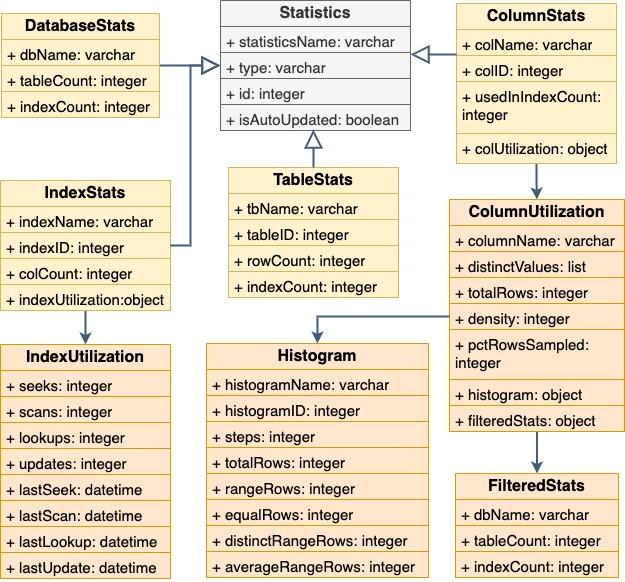
\includegraphics[width=\linewidth]{uml-db-statistic}
	\caption{A UML Class Diagram for building DBS Ontology.}
	\label{statistics-class-diagram}
\end{figure}

\subsection{Data Processing}

\subsubsection{Creation of DBS Ontology}
The initial step involves creating an ontology for DBS, focusing on columns and indexes. This is achieved through the following process:

UML to XML Conversion: Based on expertise in SQL Server, the ontology is first designed using UML diagrams. This model is then manually converted into XML format and represented using OWL (Web Ontology Language).
Visualization and Validation: The OWL and XML code are composed using a text editor, and WebVOWL is utilized to validate and visualize the ontology graph. This ontology serves as the framework for developing ontology graphs tailored to specific target schemas.

\subsubsection{Generation of Enriched DB Ontology Graphs}
Following Noy and McGuinness's guideline that “there is no one correct way to model a domain,” our methodology includes:

Data Collection and Transformation: Scripts are employed to collect and transform data from schema tables into RDF OWL formatted files. Python scripts play a crucial role in this process, including generating an HTML file for visualization.
Visual Representation: The final ontology graphs, enriched with data, are visualized and analyzed using WebVOWL, as depicted in Figure 6, which outlines the high-level workflow.

\subsubsection{Extraction of Metadata to OWL/XML}
Metadata, including tables, columns, relationships, and enriching data, are extracted and transformed into OWL format using Python scripts and JDBC connections to the SQL Server instance. This process involves wrapping and writing the data into XML files, with additional data mining logic applied for deeper insights as needed.

\subsubsection{Visualization and Evaluation}
The ontology graph is further evaluated using WebVOWL to ensure accuracy and completeness. The visualization process includes:

Accuracy Check: Verifying the ontology graph for correctness.
Enrichment Assessment: Assessing the added data to confirm its relevance and utility.
Function Utilization: Employing features such as collapse and re-evaluate as necessary to refine the ontology.

\subsection{Plan for Experimentation and Evaluation}
The objective is to build a semi-automated way to construct ontology for DB statistics, as a priliminary work for a full automated method. Thus, we will not only develop specific applications according to the use cases in section 3 in order to demonstrate the neccesity of it, but also evaluate the overall workflow, which will at least contain the following parts.

\begin{itemize}
\item Evaluation/Review of the statistics ontology setup and execution
\item Collect base data and no enriching data for column statistics simulated.
\item Evaluation of ontology graph produced in the last steps, allowing enriched data.
\item Collection of index utilization statistics, and generation of HTML enriching data.
\item Generation of index-oriented statistics ontology on target schema.
\item Evaluation of the accuracy and completeness of the generated DBS ontology.
\end{itemize}

\section{Conclusion / Future Work}
This research produce the intended ontology for DBS in XML format,
using OWL, and display via WebVOWL. The ontology is used as a framework
to creating a process that collect, transform, and extract data to XML files, producing statistics-centric ontologies. The generated ontologies included graphs of column-based statistics, index utilization statistics, and supporting HTML documents with enriching data. Further efforts may work toward improving and formalizing the ontology such that it can be used practically as a standard resource ontology. Other ontologies exist as standard and are referenced (there were several used by the generated ontologies in this research). After refinement and formalization, the ontology could be an official reference; including additional subject matter experts to review may give additional insight and refinement. Next, continuing to pursue efforts with machine learning/AI by creating an application to extract/consume/use the data is highly recommended, possibly in artificial intelligence or other technology for decisioning. 

Use of AI/ML technologies to analyze the statistics and identify data skew, troublesome statistics, or inefficient indexes may lead to better insights and database/query engine improvement. AI/ML most likely has more logic, processing, and learning capabilities than current methods and techniques; processes could be developed for deeper analysis and mining of the histograms and index utilization. Third, advancing research with current RDBMS metadata for additional opportunities and information may enhance the ontology or offer opportunities to roll up information. Finally, research may move one step further with standardization of ontology by expanding to other types of database management system (DBMS) platforms, such as NoSQL, or Graph DB. 

%%
%% The acknowledgments section is defined using the "acks" environment
%% (and NOT an unnumbered section). This ensures the proper
%% identification of the section in the article metadata, and the
%% consistent spelling of the heading.

%%
%% The next two lines define the bibliography style to be used, and
%% the bibliography file.
\bibliographystyle{ACM-Reference-Format}
\bibliography{sample-base}


%%
%% If your work has an appendix, this is the place to put it.

\end{document}
\endinput
%%
%% End of file `sample-sigconf.tex'.
